\documentclass[10pt,oneside,a4paper]{article}
\usepackage[left=2cm,right=2cm,top=2cm,bottom=1cm,includeheadfoot]{geometry}
\usepackage{ngerman}
\usepackage[utf8]{inputenc}
% \usepackage{amsfonts,amssymb,amsmath,cancel,graphicx,textcomp}
\usepackage{amsfonts,amssymb,amsmath,graphicx,textcomp}
\usepackage{float}
\usepackage{color,xcolor}
\usepackage{url}
\usepackage{hyperref}
\usepackage{listings}
\usepackage{tikz}
\usepackage{fancyhdr}
\usepackage{gensymb}
\usepackage[section]{placeins}
\usetikzlibrary{arrows,shapes,snakes,automata,backgrounds,petri,positioning}

\hypersetup{
    colorlinks,
    citecolor=black,
    filecolor=black,
    linkcolor=black,
    urlcolor=black
}

\pagestyle{fancy}
\fancyhf{}
\fancyhead[L]{crash override : \\Steve Dierker, Semjon Kerner, Artur Jeske}
\fancyhead[C]{"Ubungsblatt 10}
\fancyhead[R]{Seite \thepage}
\renewcommand{\headrulewidth}{0.5pt}

% lstlisting mit Zeilennummerierung und grauen Kommentaren, Zeilenumbruch, etc. pp.
\lstset{
  numbers=left, numberstyle=\tiny, numbersep=5pt,
  tabsize=2,
  breaklines=true, breakindent=0pt, postbreak=\mbox{$\rightarrow\ \ $},
  showstringspaces=false,
  extendedchars=false,
  basicstyle=\small\ttfamily,
  commentstyle=\color{black!40},
  stringstyle=\color{black!40!blue},
  keywordstyle=\color{black!40!green}
}

% Komma Abstände bei Tausendern/Dezimalzahlen ans dt. anpassen
\mathcode`,="013B
\setlength{\parindent}{0em}
\setlength{\parskip}{0.5em}

\begin{document}
	Die erste Aufgabe ist uns nicht gelungen und daher konnten wir für die zweite Aufgabe
    nur eine Idee Implementieren und nicht austesten.
  \section{Closest Point with Prediction}
    \begin{figure}[h]
      \centering
      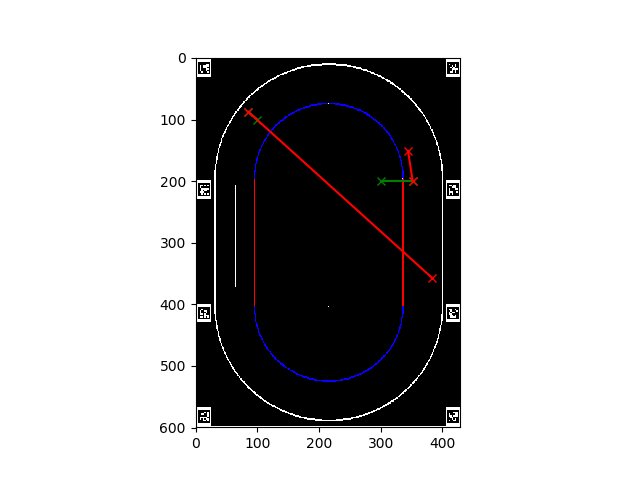
\includegraphics[scale=0.7]{pictures/ass10_1.png}
      \caption{Karte mit nächsten Punkten (grün) und errechneten Distanzen (rot)}
    \end{figure}
    \url{https://github.com/bigzed/model_car/blob/version-4.0/texinput/src/closest_distant_point.py} \\
    Das Konzept, dass wir in dieser Aufgabe versucht haben umzusetzen basiert auf
    der Aufgabenstellung der vorangegangen Woche. Dazu wird zunächst ein closest point
    zu einem Punkt berechnet. Dieser ist nun zusätzlich abhängig von der laneID, indem
    die innere Spur eine Vergrößerung des Ovals um 16 cm und die äußere um 48 cm erhält. \\
	
	Nun wird die Distanz zusätzlich hinzugefügt, für eine Gerade ist dies trivial, sollte
	jedoch der Bereich zuende sein und es ist noch etwas von der Distanz übrig, dann
	wird der Rest auf den anschließenden Kreis abgebildet. \\
	
	Beim Abbilden auf den Kreis hatten wir keinen Erfolg. Unser Vorgehen:
	\begin{enumerate}
		\item Den gefunden Closest Point um den Kreismittelpunkt in Richtung des
		Koordinatenursprung verschieben
		\item Herausfinden des Winkels des Closest Points
		\item Errechnen des Winkels der Distanz auf dem Kreis
		\item Rotieren des Vektors des Closest Points mittels Drehmatrix um die Summe der
		beiden Winkel.
		\item Abziehen und merken der möglichen Distanz, die den Halbkreis überschreitet.
		\item Verschieben des Vektors des Closest Points (bereits rotiert um den Winkel der
		Distanz) zurück in Richtung des ursprünglichen Kreises.
	\end{enumerate}
	Zu beobachten ist, dass umso größer der Winkel, umso größer wird die Distanz
	abgebildet. Dies ist gut zu vergleichen an den beiden Punkten im Bild. \\
	Der Punkt rechts oben ist 0°, während der Punkt links oben zwischen 90° und 180° eine
	unwahrscheinlich hohe Distanz bekommt. Dies konnten wir uns nicht erklären, da es 
	augenscheinlich nicht mehr von dem Distanzwert, sondern von dem Winkel abhängig wurde.
	\newpage
  \section{Follow lane with ceiling camera GPS}
    \url{https://github.com/bigzed/model_car/blob/version-4.0/catkin_ws/src/assignment10_look_ahead_point_and_gps/src/line_detection.py}\\
	Da wir nur Konzepte implementieren konnten, wird folgend die Grundidee am Code erklärt.
	\begin{itemize}
		\item In Zeile 86 wurde die Fehlerübergabe für die Lenkung auf die GPS-Lokalisierung umgestellt.
		\item In den Zeilen 245-251 wurde das Quaternion in die Ausrichtung (yaw)
		des Fahrzeugs transformiert.
		\item In den Zeilen 252-258 wurde der Fehler aus dem Winkel zwischen Blickrichtung
		des Fahrzeugs und Winkel des Fahrzeugs zum entfernten Punkt ermittelt.
	\end{itemize}
\end{document}
